\documentclass[english,authoryear,12pt]{elsarticle}
%%%%%%%%%%%%%%%%%%%%%%%%%%%%%%%%%%%%%%%%%%%%%%%%%%%%%%%%%%%%%%%%%%%%%%%%%%%%%%%%%%%%%%%%%%%%%%%%%%%%%%%%%%%%%%%%%%%%%%%%%%%%%%%%%%%%%%%%%%%%%%%%%%%%%%%%%%%%%%%%%%%%%%%%%%%%%%%%%%%%%%%%%%%%%%%%%%%%%%%%%%%%%%%%%%%%%%%%%%%%%%%%%%%%%%%%%%%%%%%%%%%%%%%%%%%%
\usepackage{fullpage}
\usepackage[labelfont=bf,singlelinecheck=false,aboveskip=10pt]{caption}
%\usepackage[font={scriptsize},labelfont={scriptsize},textfont={scriptsize}]{caption}
%\DeclareCaptionFormat{myformat}{#1#2\\#3}
\usepackage{amsmath,graphicx,multicol,chngpage,setspace}
\usepackage{amssymb,amsthm,amstext,amsfonts,enumerate}
\usepackage[colorlinks=true,linkcolor=black, citecolor=blue, urlcolor=blue]{hyperref}
\usepackage[top=1in, bottom=1in, left=1.0in, right=1.0in]{geometry}
\usepackage{lscape}
\usepackage{rotating}
\usepackage{color,float,multirow,array,hyphenat}
\usepackage{booktabs}
\usepackage{subcaption}
\usepackage{natbib} % already loaded by elsarticle
\usepackage{apalike}
\usepackage{babel}
\usepackage{appendix}
\usepackage{afterpage}


\setcounter{MaxMatrixCols}{10}

% Global Document settings
%\graphicspath{{C:/Work/Papers/Murray/Projects/AIT/ait-ahmad-murray/paper/Images}}
% \linespread{1.3} % Setting it to 1.3 = 1.5 line spacing; 1.6 = double spacing
\onehalfspacing
\setlength{\parindent}{0in}
\setlength{\parskip}{1em}

% Create arg max/min operator
\DeclareMathOperator*{\argmax}{arg\,max}
\DeclareMathOperator*{\argmin}{arg\,min}
\DeclareMathOperator{\E}{\mathbb{E}}

\newcommand{\bi}{\begin{itemize}}
\newcommand{\ei}{\end{itemize}}
\newcommand{\be}{\begin{enumerate}}
\newcommand{\ee}{\end{enumerate}}
\newcommand{\bd}{\begin{description}}
\newcommand{\ed}{\end{description}}
\newcommand{\prbf}[1]{\textbf{#1}}
\newcommand{\prit}[1]{\textit{#1}}
\newcommand{\beq}{\begin{equation}}
\newcommand{\eeq}{\end{equation}}
\newcommand{\beqa}{\begin{eqnarray}}
\newcommand{\eeqa}{\end{eqnarray}}
\newcommand{\bdm}{\begin{displaymath}}
\newcommand{\edm}{\end{displaymath}}
\newcommand{\script}[1]{\begin{cal}#1\end{cal}}
\newcommand{\citee}[1]{\citename{#1} \citeyear{#1}}
\newcommand{\h}[1]{\hat{#1}}
\newcommand{\ds}{\displaystyle}


% Remove Elsevier preprint message
\makeatletter
\def\ps@pprintTitle{%
	\let\@oddhead\@empty
	\let\@evenhead\@empty
	\def\@oddfoot{}%
	\let\@evenfoot\@oddfoot}
\makeatother

\begin{document}
%	\begin{frontmatter}
%		\title{Implications for Determinacy with Average Inflation Targeting}
%		\date{\today}
%		\author[1]{Yamin Ahmad \corref{cor1}}
%		\ead{ahmady@uww.edu}
%		\author[2]{James Murray}
%		\ead{jmurray@uwlax.edu}
%
%		\cortext[cor1]{Corresponding author}
%		\address[1]{Dept. of Economics, University of Wisconsin - Whitewater, 809 W. Starin Road, Whitewater, WI 53190, USA}
%		\address[2]{Dept. of Economics, University of Wisconsin - La Crosse, 1725 State St., La Crosse, WI 54601, USA}
%
%	\date{\today}
%
%	\begin{abstract}
%		%\renewcommand{\baselinestretch}{1.5}
%		We use a standard New Keynesian model to explore implications of backward- and forward-looking windows for monetary policy with average inflation targeting and investigate the conditions for determinacy. A unique equilibrium rules out sunspot shocks that can lead to self-fulfilling shocks for inflation expectations. We find limitations for the length of the forward window and demonstrate how this depends on other parameters in the model, including parameters governing monetary policy and expectations formation.
%
%		\begin{flushleft}
%			{\it JEL Classification}: E50, E52, E58 \newline
%			{\it Keywords}: Average Inflation Targeting, Determinacy, Monetary Policy
%		\end{flushleft}
%	\end{abstract}
%
%\end{frontmatter}

%\renewcommand{\baselinestretch}{2.0}
\renewcommand{\thefootnote}{\arabic{footnote}}%
\setcounter{page}{1}%
\setcounter{footnote}{0}%


\section{\label{Intro}Introduction}
In 2020, the Fed laid out an average inflation targeting (AIT) monetary policy framework where inflation could temporarily deviate from the Fed's target in the short run, as long as the average level of inflation in the medium to long run remained consistent with the Fed's target. If inflation remained consistently below its target for some period, it could be followed by a period where inflation would remain above its target.

Recent research has been examining a range of issues related to AIT, including welfare implications (e.g. \citealp{budianto2020}; \citealp{eo2020}), how AIT affects inflation expectations (e.g. \citealp{coibion2020}; \citealp{hoffmann2022}), and implications for boundedly-rational expectations on macroeconomic outcomes (eg: \citealp{honka2021}; \citealp{budianto2020}). A central question that pertains to the literature on the AIT framework is the window for how the `average' level of inflation is determined. It may be based purely on past values of inflation, expectations of future values for inflation, or some combination.

We examine this issue within the context of a standard three-equation New Keynesian model. We construct a measure of the inflation target that is a weighted average of past observations of inflation, current inflation, and expectations for future values of inflation. We evaluate conditions on monetary policy and the target window to assure determinacy. With indeterminacy, the economy is subject to sunspot shocks, where self-fulfilling expectation shocks can lead to excess volatility in the business cycle (see, for example, \citealp{lubik2004}).

\section{\label{Model}Model}
This paper builds upon a standard three-equation New Keynesian model along the lines of \cite{clarida1999}.

\subsection{Baseline Framework}

The IS equation is derived from consumer utility maximization and states that the current output gap depends on expectations of next period's output gap, and is negatively related to the real interest rate:
\begin{equation}\label{eq:ISe}
	x_t = x_{t+1|t}^e - \frac{1}{\sigma} \left( r_t - \pi_{t+1|t}^e  - r^n  \right) + \xi_t^{x},
\end{equation}
where $x_t$ denotes the output gap (given by the difference between the log of output and its natural rate), $r_t$ is the nominal interest rate, $\pi_t$ the inflation rate, $r^n = 1/\beta - 1$ the natural rate of interest and $\beta \in (0,1)$ is the household's discount factor, and $x_{t+1|t}^e$ and $\pi_{t+1|t}^e$ represent private sector expectations on next period's output gap and inflation rate, respectively. The preference parameter, $\sigma$, is inversely related to consumers' intertemporal elasticity of substitution, and $\xi_t^x$, represents a demand shock. A fraction of agents, $\lambda\in[0,1)$, form na\"ive expectations, so aggregate expectations are given by,
\begin{equation}
	\begin{array}{c}
		x_{t+1}^e = \lambda x_t + (1-\lambda) \E_t x_{t+1}, \\ [1.5pc]
		\pi_{t+1}^e = \lambda \pi_t + (1-\lambda) \E_t \pi_{t+1}. \\
	\end{array}
\end{equation}
Expectations are fully rational when $\lambda=0$. We explore the implications for indeterminacy when not all agents are fully rational.

The second equation is the Phillips Curve which states that inflation depends on the expectation of next period's inflation and the output gap:
\begin{equation}\label{eq:PhillipsCurvee}
	(\pi_t - \pi^*) = \beta (\pi_{t+1|t}^e - \pi^*) + \kappa x_t + \xi_t^{\pi},
\end{equation}
where $\pi^*$ is the long-run steady state inflation rate, $\xi_t^\pi$ is an exogenous cost shock, and $\kappa$ is a reduced form parameter that is inversely related to the degree of price stickiness.\footnote{In a typical model, $\kappa=(1/\omega)(1-\omega)(1-\omega\beta)$, where $\omega \in (0,1)$ is the fraction of firms that do not re-optimize their prices each period. \citet{smetswouters2007} estimate $\omega \approx 0.66$.}

The third relationship governs monetary policy:
\begin{equation}\label{eq:TaylorRule}
	r_t = (1-\rho_r)(r^n + \pi^*) + \rho_r r_{t-1} + (1-\rho_r) \left[ \psi_\pi (\pi_t^A - \pi^*) + \psi_x x_t \right] + \epsilon_t^{r},
\end{equation}
where $\rho_r$ captures persistence, and $\psi_\pi$ and $\psi_x$ represent policy responses to inflation and the output gap, respectively. The average inflation target is given by $\pi_t^A$ and $\epsilon_t^r$ is a monetary policy shock.

\subsection{Average Inflation Targeting}

Monetary policy targets an average value of inflation over a target window that may include backward- and forward-looking terms for inflation. The average inflation target is:
\begin{equation}
	\pi_t^A = \gamma \pi_t^B + (1-\gamma) \pi_t^F,
\end{equation}
where $\gamma \in [0,1]$ is the relative weight given to past average inflation, $\pi_t^B$, versus expected future average inflation, $\pi_t^F$. The past average inflation is given by,
\begin{equation}\label{eq:backward}
	\pi_t^B = \delta_B \pi_t + (1-\delta_B) \pi_{t-1}^B,
\end{equation}
where $\delta_B \in (0,1)$ is the weight given to the most recent observation. We include the current value for inflation, $\pi_t$, in this ``backward-looking" window.  Repeated substitution reveals the nature with which the weights decline geometrically with time:
\begin{equation}\label{eq:backward_all}
	\pi_t^B = \delta_B \sum_{j=0}^{\infty} (1-\delta_B)^j \pi_{t-j},
\end{equation}
where $\delta_B (1-\delta_B)^j$ is the weight on an observation of inflation $j$ periods in the past, $\sum_j \delta_B (1-\delta_B)^j=1$, and $\lim_{j \to \infty} \delta_B (1-\delta_B)^j=0$. Smaller values for $\delta_B$ can be viewed as longer backward-looking windows for average inflation targeting and a weight of $\delta_B$ approximates monetary policy behavior using an equally-weighted finite window of length $1 / \delta_B$ periods. Similarly,
\begin{equation}\label{eq:forward}
	\pi_t^F = \delta_F \E_t \pi_{t+1} + (1-\delta_F) \E_t \pi_{t+1}^F,
\end{equation}
where $\delta_F \in (0,1)$ is the weight given to next period's expected inflation. The forward-looking average is a sum of only expected future outcomes. Repeated substitution reveals,
\begin{equation}\label{eq:forward_all}
	\pi_t^F = \delta_F \sum_{j=0}^{\infty} (1-\delta_F)^j E_t \pi_{t+1+j},
\end{equation}
where the weight on expected inflation rate $j$ periods in the future, $\delta_F (1-\delta_F)^{j}$, declines geometrically with the distance into the future, $\sum_j \delta_F (1-\delta_F)^{j}=1$, and $\lim_{j \to \infty} \delta_F (1-\delta_F)^j=0$. The value $1/ \delta_F$ approximates the length of an equally-weighted finite forward-looking window. We vary the parameters $\left\{\delta_B, \delta_F, \gamma, \lambda, \psi_\pi, \psi_x, \rho_r \right\}$ and explore the implications for determinacy below. Note that a standard Taylor-type rule emerges as a special case with $\gamma=1.0$ and $\delta_B=1.0$.

\subsection{Full Model}

Following \citet{sims2002}, the model can be expressed as,
\begin{equation}
	\Gamma_0 y_t = \Gamma_1 y_{t-1} + \Psi z_t + \Pi \eta_t
\end{equation}
where $y_t$ is a vector that includes $x_t$, $\pi_t$, $r_t$, $\pi_t^A$, $\pi_t^B$, and $\pi_t^F$; $z_t$ is a vector of the shocks, $\xi_t^x$, $\xi_t^\pi$, and $\xi_t^r$; and $\eta_t \equiv y_t - E_{t-1} y_t$ equals the ex-post rational expectations forecast errors. We use the method in \citet{sims2002} to explore regions of indeterminacy.

\begin{table}[htp]
	\captionsetup{justification=centering}
	\caption{Parameter Calibrations}\label{tb:parms}
	\begin{center}
		\vspace*{-1pc}\begin{tabular}{lcr}
			Description & Parameter & Value \\ \hline
			Discount rate (quarterly) & $\beta$ & 0.99 \\
			Inverse intertemporal elasticity & $\sigma$ & 0.72 \\
			Phillips curve coefficient & $\kappa$ & 0.178 \\
			Steady state inflation rate (quarterly) & $\pi^*$ & 0.005 \\ [0.25pc]
			\hline \\ [-0.25pc]
			Baseline Parameters & Parameter & Value(s) \\ \hline
			AIT weight past inflation & $\gamma$ & $\left\{ 0.0, 0.25 \right\}$ \\
			Backward-looking weight & $\delta_B$ & 1.0 \\
			Monetary policy: average inflation & $\psi_\pi$ & 1.5 \\
			Monetary policy: output gap & $\psi_x$ & 0.5 \\
			Monetary policy: persistence & $\rho_r$ & 0.0 \\ \hline
		\end{tabular}
	\end{center}
\end{table}

Parameter calibrations are given in \href{tb:parms}{Table} \ref{tb:parms}. Values for $\sigma$ and $\kappa$ are set to estimates from \citet{smetswouters2007}. We set $\pi^*=0.005$ so that the annualized long-run inflation level is 2\%.

We explore the determinacy regions for $\delta_F$, the weight placed on the expected value for the next period's inflation in the forward-looking window. We investigate how the regions of determinacy differ with calibrations for the weight placed on past inflation in the AIT window, $\gamma$; the weight placed on the most recent inflation observation in the backward-looking window, $\delta_B$; and the Taylor rule coefficients, $\psi_\pi$, $\psi_x$, and $\rho_r$. The baseline parameters given in \href{tb:parms}{Table} \ref{tb:parms} represent the calibrations we use when not varying each of those particular parameters. We use $\gamma=0.0$ for all calibrations not involving the backward-looking parameter, $\delta_B$, implying monetary policy is purely forward looking. When exploring determinacy ranges for $\delta_B$, we use a weight $\gamma=0.25$. We set the baseline values for $\psi_x=0.5$, $\psi_\pi = 1.5$, and $\rho=0.0$.

\section{Results}

\begin{figure}
	\captionsetup{justification=centering}
	\begin{center}
		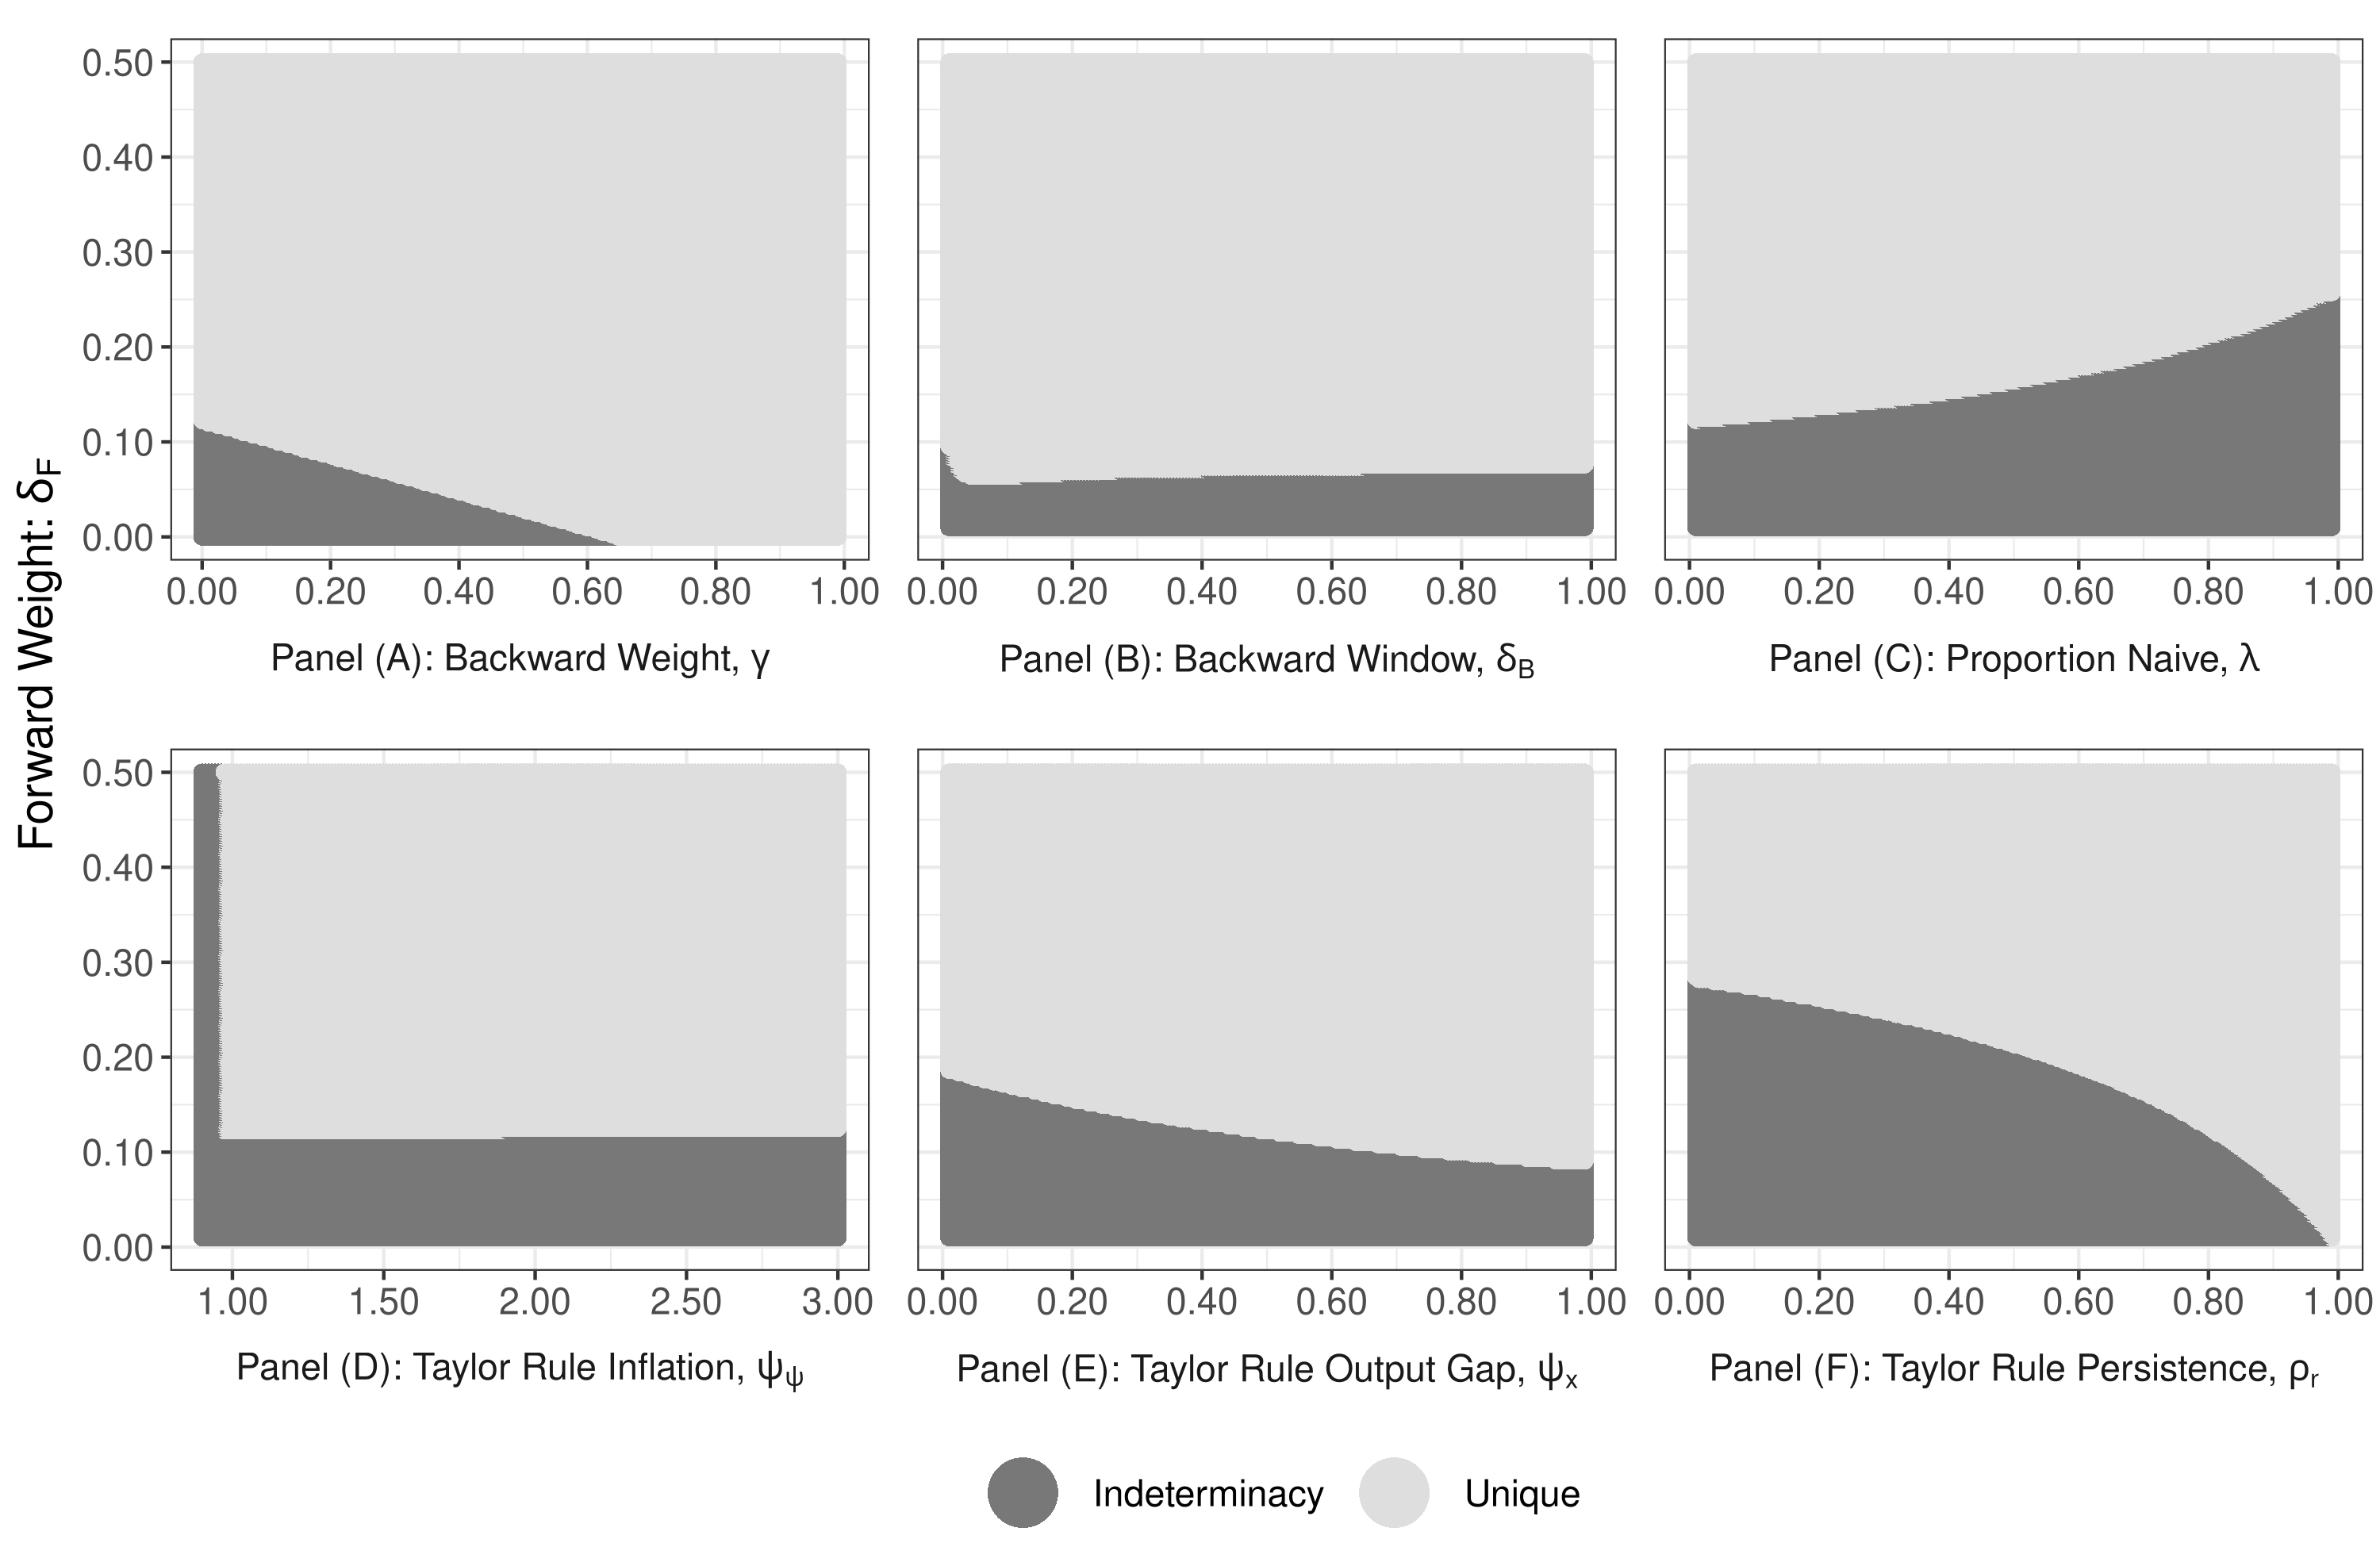
\includegraphics[width=\textwidth]{./determinacy_notitle.png}
		\vspace*{3pc}\hspace*{2pc}\parbox{0.9\textwidth}{\small{
			Notes: Parameters not varying in each graph are given in \href{tb:parms}{Table} \ref{tb:parms}. In Panel (B), the baseline parameter for $\gamma$ is 0.25, implying a 25\% weight given to the backward-looking window. In all other panels, $\gamma$ is set to 0.0, implying purely forward-looking windows.}
		}
	\end{center}
	\vspace*{-4pc}\caption{Regions of Determinacy for Forward-Looking Windows}\label{fg:determinacy}
\end{figure}

\href{fg:determinacy}{Figure} \ref{fg:determinacy} shows the regions of determinacy for different values of the forward-looking weight, $\delta_F$, depending on four other parameters in the model. Given the inverse relationship between the weight on an individual observation and the length of a finite window, larger values for $\delta_F$ imply shorter forward-looking windows. The largest value considered, 0.5, approximates a two-quarter window.

Panel (A) demonstrates the importance of using current or past values inflation in the target window. When $\gamma=0.0$, no weight is put on past or current inflation, and the window is purely forward-looking. The smallest value for $\delta_F$ that delivers determinacy in this scenario is 0.28, so the largest possible forward-looking window is approximately 3.57 quarters. When $\gamma \geq 0.63$, all possible forward-looking windows yield determinate solutions. This implies, though, that the target window has at least a 63\% weight on the current inflation rate, and therefore at most a 37\% weight on future inflation.

Panel (B) shows how the length of the backward-looking window affects determinacy. The minimal combinations of values for $\delta_B$ and $\delta_F$ that achieve determinacy are each 0.14, implying the longest the forward-looking and backward-looking windows can be are approximately 7.14 quarters. Panel (C) reveals that the presence of na\"ive agents have crucial implications for determinacy. When more than 40\% of agents form na\"ive expectations, no purely forward-looking window for AIT leads to determinacy.

Panels (D), (E), and (F) show how the length of the forward-looking window depends on the Taylor Rule coefficients. Larger response to inflation lead to more restrictive forward windows. Larger responses to the output gap are necessary are also important for determinacy. Values of $\psi_x \geq 0.2$ are necessary and larger values allow for longer forward windows.  Monetary policy persistence can play an important role. The stronger is persistence, the longer can be the forward looking window.

\section{Conclusion}

Forward-looking AIT has important implications for monetary policy to avoid issues of indeterminacy. We find large ranges of indeterminacy, especially when a large portion of aggregate expectations are na\"ive, when little weight is put on the output gap, and when the forward window is greater than two years. Our findings suggest that the Fed can assure determinacy with a high rate of monetary policy persistence or with a target window that puts significant weight on current and past inflation.

\bibliographystyle{apalike}
\bibliography{ait}

\end{document}
